\section{Results}
Associations of Food Groups, Food Subgroups, Food Nutrients with CKD mortality as discovered by the experiments above are provided in this section. Outcome of ACR value prediction in the test data are also provided.

\subsection{Food Groups, Food Subgroups, Food Nutrients and CKD Mortality}
\noindent \textbf{Food Groups and Mortality}

\noindent Experiments (Set 1 ) with aggregated NHANES and USRDS  data to find associations between food groups and CKD mortality using PCA and Regression show that Grains (-0.84) and Fruits (-0.43) have negative correlations with CKD mortality i.e. mortality is high for the patients who took significantly lower amount of Grains and Fruits than recommended amounts. Data exploration (plots below) also reflects the negative relation. As the correlation for fruits is -0.43 i.e. not very high, hence, Fruits can be thought of mildly/moderately associated.
\begin{figure}[!htb]
\small
\begin{tabular}{cc}	
\specialcell{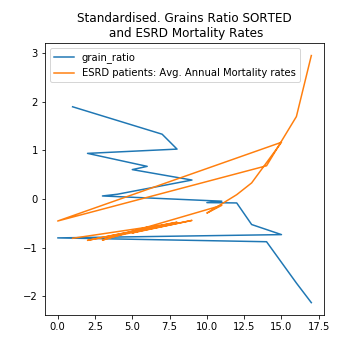
\includegraphics[scale=0.25]{sorted_standard_grain_ratio_negative.png}  }  &  \specialcell{ 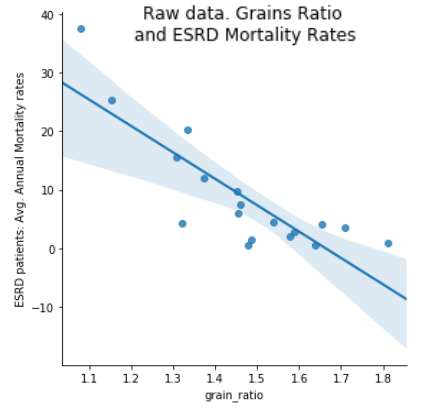
\includegraphics[scale=0.25]{grain_later.png} } \\
Grains & Grains \\
\end{tabular}
\centering
\vspace{0.25cm}
\begin{tabular}{cc}	
\specialcell{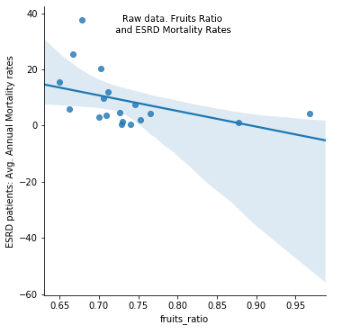
\includegraphics[scale=0.3]{pair_plot_fruits_ratio} } & \specialcell{ 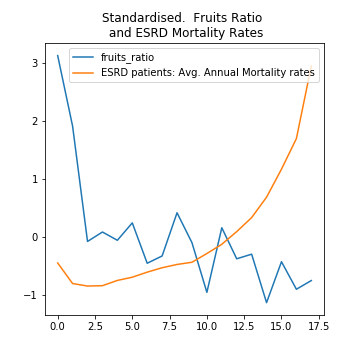
\includegraphics[scale=0.25]{standard_fruit_ratio_mortality.png} } \\
Fruits & Fruits \\
\end{tabular}
\caption{\textbf{Food Groups and Mortality - Negative Correlations}}
\vspace{0.25cm}
\end{figure}

\begin{figure}[!htb]
\small
\begin{tabular}{cc}	
	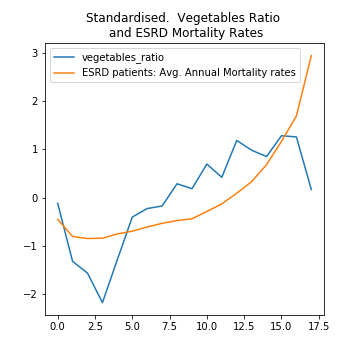
\includegraphics[scale=0.25]{standard_vegetable_ratio.png} & 
	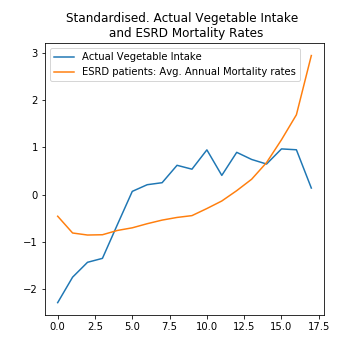
\includegraphics[scale=0.25]{standard_actual_vegetable_intake_esrd_mortality.png}\\
	\multicolumn{2}{c} { 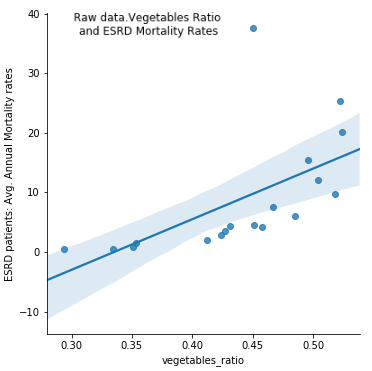
\includegraphics[scale=0.25]{pairplot_vegetable_.png}} 	  \\
	\multicolumn{2}{c}{Vegetables Ratio}  \\ 
\end{tabular}
\centering
\caption{\textbf{Food Groups and Mortality - Positive Correlations (Vegetables) }}
\end{figure}

\noindent Vegetables show positive (0.58) correlation i.e. mortality is high for the patients who took more vegetables. The correlation of 0.58 does not provide a very strong conclusion. Data shows such correlations in older adults. Even though ratios of food intake amount to high end of recommended amounts (actual intake amounts also show positive relation) were used; age might have biased the correlation. This does not show conformity with the general recommendation to take more vegetables for CKD patients. However, as experiments with food subgroups show that vegetable subgroups such as Other vegetables (0.68), Red and Orange vegetables (0.55), and Starchy vegetables (0.44) show positive correlations that have an impact on the Vegetable group correlation.  Although more vegetable intake is a general recommendation for CKD patients, certain vegetables with more carbohydrates (and sugars) such as Starchy Vegetables as well as Vegetables with more Potassium and Calcium such as Tomatoes, and Spinach are recommended to be taken at a lower amount. For diabetes induced CKD, starchy vegetables are not highly recommended in general. Considering the subgroups, the moderate positive correlation as this study found for vegetables food group is in conformity with the general recommendations for CKD patients.

\noindent Experiments (Set 2) with aggregated NHANES and USRDS data to find associations between food subgroups and CKD mortality using PCA and Regression show that  Other vegetables (0.68),    Red and orange vegetables (0.55), and Starchy vegetables (0.44)  have positive correlations with mortality i.e. mortality is low when the intake amounts are low, and mortality is high when intake amounts are high. Data Exploration plots as given below also show these positive relations.

\noindent  Food subgroups such as Alcoholic Beverages (-0.79),    Added Sugars/Sugars and Sweets (-0.64), Whole Grains (-0.61), and  `Nuts, Seeds, and Soy Products' (-0.55) show the most negative correlations with CKD mortality. Data exploration also shows negative correlations as shown in the charts below. These outcomes are also consistent with current knowledge except for Sugars. Prevalence of Stage 3 CKD is lower in Alcohol Drinkers than non-drinkers [2, 49], Nuts being Phosphorus rich and Whole Grains being Potassium rich are detrimental to CKD patients and can cause higher mortality when taken in higher quantities.

\begin{figure}[!htb]
\small
\begin{tabular}{cc}
	\specialcell{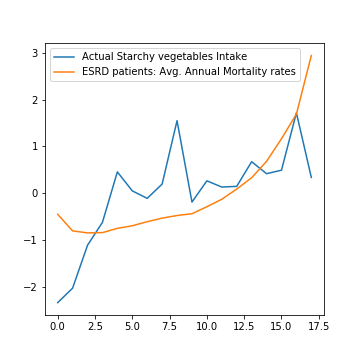
\includegraphics[scale=0.25]{standard_actual_starchy_vegetable_esrd_mortality.png} \\  Starchy Vegetables } & 
	\specialcell{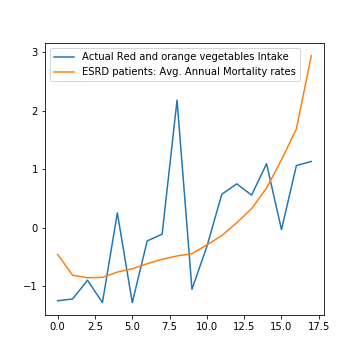
\includegraphics[scale=0.25]{standard_actual_red_and_orange_vegetable_esrd_mortality.png} \\ Red and Orange Vegetables } \\
	 \multicolumn{2}{c} { \specialcell{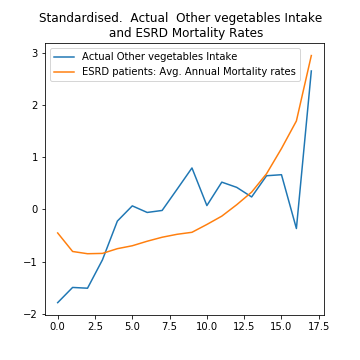
\includegraphics[scale=0.25]{standard_actual_other_vegetable_esrd_mortality.png}	\\ Other Vegetables } } \\
\end{tabular}
\centering
\caption{\textbf{Food Subgroups and Mortality - Positive Correlations}}
\begin{tabular}{cc}
	\specialcell{ 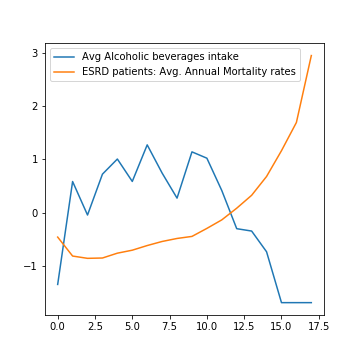
\includegraphics[scale=0.25]{negatively_subgroup_avg_alcohol_intake}  \\   Alcohol Intake  }  & 
	\specialcell{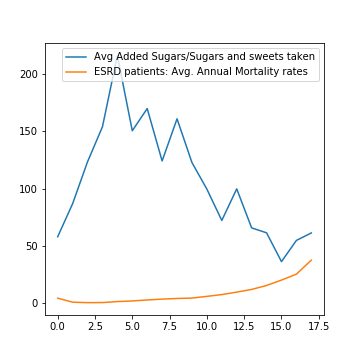
\includegraphics[scale=0.25]{negatively_added_sugar_subgroup_line_2}   \\  Sugar }  \\
	
	\specialcell{ 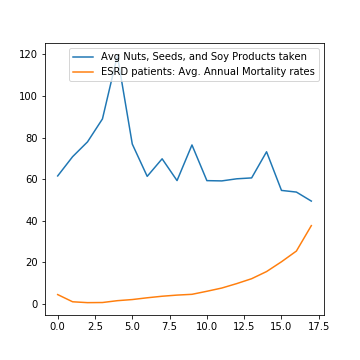
\includegraphics[scale=0.25]{negatively_avg_nuts_subgroup_line_3}  \\ Nuts, Seeds } &
	\specialcell{ 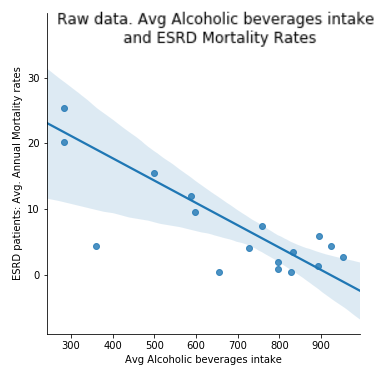
\includegraphics[scale=0.25]{pairplot_avg_alc.png}  \\ Alcohol } \\
	
	\specialcell{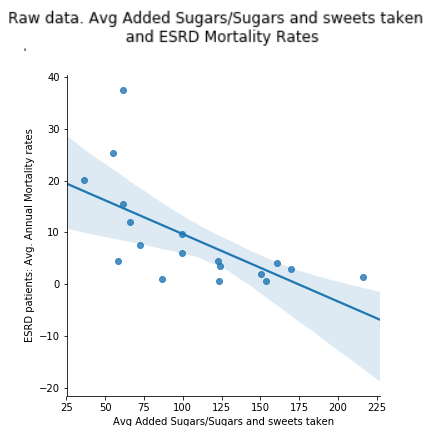
\includegraphics[scale=0.25]{pairplot_raw_data_added_sugar_esrd}  \\ Added Sugar } &
	\specialcell{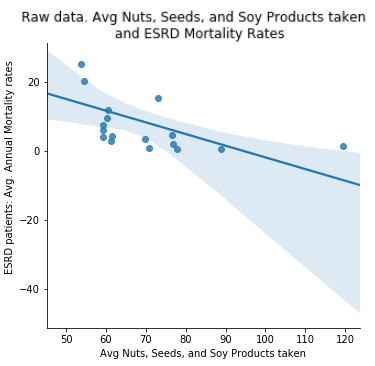
\includegraphics[scale=0.25]{pairplot_nuts_avg_negative.png}  \\ Nuts, Seeds } \\
\end{tabular}
\centering
\caption{\textbf{Food Subgroups and Mortality - Negative Correlations}}
\end{figure}

\noindent \textbf{Mortality Study with Non-aggregated Data}

\noindent For experiments (Set 7) where mortality rates based on ages were used for each NHANES survey row (i.e. not aggregated), the following food subgroups show more positive correlations than others: Fats, Eggs, Other vegetables, Nonalcoholic beverages, White potatoes and Puerto Rican starchy vegetables, Tomatoes and tomato mixtures, Oils, Deep-yellow vegetables respectively. In the study, the following subgroups showed more negative correlations than others: Grain mixtures, Frozen plate meals, Soups, Crackers and Salty snacks from grain products, Milks and milk drinks, Sandwiches with Meat, Poultry, and fish, Poultry. Although the correlation numbers in this study are very low, the positive and negative correlations are consistent with current knowledge [48, 49, 50, 51, 52, 53, 54, 55, 56, 57].

\begin{table}[!htb]
\caption{\textbf{Outcome when ACR Values are used as the Target}}
\label{outcome-acr-values}
\vspace{0.25cm}
\small
\begin{tabular}{ | p{1.1cm} | p{1.1cm} | p{1.45cm} | p{0.9cm} | p{0.9cm} | p{1.5cm} | }
\hline
\specialcell{ \textbf{Data} \\ \textbf{Normal} \\\textbf{ized}}	& 
\textbf{Target}	&  
\textbf{Approach}	&  
\specialcell {\textbf{MSE} \\ \textbf{Train} }	&  
\specialcell { \textbf{MSE} \\ \textbf{Test}}	&  
%\specialcell {\textbf{RMSE} \\ \textbf{Train}}	&  
%\specialcell { \textbf{RMSE} \\ \textbf{Test}}	&  
%\specialcell {\textbf{R2} \\ \textbf{Score} \\ \textbf{Train}} &  
\specialcell {\textbf{Accuracy} } \\

%\\ \textbf{Test R2} \\ \textbf{Score} \\ \textbf{if not} \\ \textbf{mentioned}

\hline
No			& 
\specialcell{ACR \\Value}	& 
\multicolumn{3}{c|} { \specialcell{10 Fold Cross Validation \\Polynomial Regression}} 		&	
%1 				& 
%2 					 & 
%3 					  &	
\specialcell{-0.957  \\ cross val \\ score } \\


\hline
No			& 
\specialcell{ACR \\ Value} 	& 
\multicolumn{3}{c|} { \specialcell{ Polynomial Bayesian \\with Cross Validation }} 		&	
%1 				& 
%2 					 & 
%3 					  &	
\specialcell{-0.682 \\ cross val \\score } \\

\hline
No			& 
\specialcell{ACR \\ Value}	& 
\specialcell { Polynomial \\ Regression }	&  
90965	& 
52946	& 
%301	& 
%301	& 
%0.359	& 
\specialcell {-0.579 \\ r2 score \\on \\test data } \\

\hline
No	& 
\specialcell{ACR \\Value}	& 
\specialcell{Bayesian on \\ Polynomial \\ fit}	& 
93047	& 
47431	& 
%305	& 
%305	& 
%0.344	& 
\specialcell {-0.414 \\ r2 score \\on \\test data }  \\
\hline
\end{tabular}
\end{table}


\noindent \textbf{Food Groups, Food Nutrients, and Albumin to Creatinine Ratio (ACR) Association}

\noindent The experiments (Set 3, 4, and 5) using PCA and Regression showed negligible correlation between ACR and food groups and subgroups intake. However, some food groups and/or nutrients such as Dairy, and  `Sugars, Sweets, and Beverages'  have higher and positive though negligible (0.02) effect than the others where Fruits (-0.01) showed negative effect.  For nutrients, Polyunsaturated fatty acids (-0.02), and Iron (-0.02) have negative correlations where Choline (0.02) showed better positive correlation than others. Findings for Choline matches with medical knowledge [48]. As the correlations are not significant further analysis can be done on the data especially for food groups and nutrients that are found important (using PCA) in the data as provided below:

\noindent Dairy,  Fats, oils, and salad dressings’,  Fruits,  Grains,  Protein,   Sugars, sweets, and beverages’, Vegetables, Avg energy kcal,  avg protein gm,  avg carbohydrate gm,  avg total fat gm,  avg total saturated fatty acids gm, avg total monounsaturated fatty acids gm,  avg total polyunsaturated fatty acids gm, avg lutein zeaxanthin mcg,  avg thiamin vitamin B1 mg,  avg riboflavin Vitamin B2 mg,  avg Niacin mg, avg Calcium mg,  avg Phosphorus mg,  avg Magnesium mg,  avg Iron mg, avg Zinc mg,  avg Copper mg,  avg Sodium mg,  avg Potassium mg,  avg Selenium mcg,  Hexadecenoic gm,  Octadecenoic gm

\subsection{Food Subgroups and Albumin to Creatinine Ratio (ACR) Association}

\noindent The experiments showed  `Milk desserts, Sauces, Gravies' (0.22), and Alcoholic Beverages (0.087) have more positive correlations with ACR than the other food subgroups  i.e. taking more of these food subgroups results higher ACR values. Research by Uehara et al. [55] also shows that excessive Alcohol consumption can cause Proteinuria/Albuminuria (high ACR). Nettleton et al. [56] found that high fat dairy can be linked to high ACR values where low-fat dairy is not strongly linked to high ACR values. However, the correlation as this research found is very low. Low values might still explain a correlation where ACR values might depend on other factors in together than only these food subgroups. Fruits and juicy baby foods show negative correlation (-0.04) though not significant i.e. taking high amount does not increase ACR values that matched with current knowledge [57].


\subsection{Predictability of ACR values based on Dietary patterns}
Experiments (Set 6 ) were conducted to predict ACR values from the dietary intake patterns data. Machine Learning (ML) Approaches of Regression, Polynomial Regression, Random Forest Regression, Bayesian prediction with or without 10 fold cross validations were applied on Food Subgroups intake dataset. Only the food subgroups that were found to be important using PCA were used for the ML approaches.

\noindent \textbf{Target Variables}

\noindent Absolute ACR values and ACR Categories were used as the target variables.  For ACR category, ACR  \textless   30 is assigned to class 0 (i.e. no ckd), and ACR  \textgreater  30 is assigned to class 1 (CKD). ACR values less than 30 indicate no CKD, where ACR values between 30 and 300 indicate moderate CKD. ACR \textgreater 300 is considered severe CKD.

\noindent \textbf{Outcome when ACR Values are used as the Target }

\noindent The best test set accuracies were found using  approaches such as: 10 Fold Cross Validations with Polynomial Regression (95\%), Polynomial Bayesian with 10 fold Cross Validations (68\%), Polynomial Regression (57\%), Bayesian on Polynomial fit (41\%), Cross Validation with Polynomial Random Forest Regression (21\%). A list of the best performing approaches and the outcome are provided in Table \ref{outcome-acr-values} below. 

\begin{table}
\caption{\textbf{Outcome when ACR Category is used as the Target}}
\label{outcome-acr-category}
\vspace{0.25cm}
\small
\begin{tabular}{ |p{1.1cm} | p{1.15cm} | p{1.5cm} | p{1.4cm} | p{1.4cm} | }
\hline
\textbf{Data Normal}	& \textbf{Target} & \textbf{Approach}	& \specialcell{\textbf{Train} \\ Confusion \\ \textbf{Matrix} }	   & \specialcell{\textbf{Test} \\ Confusion \\ \textbf{Matrix} } \\
\hline
No		& Category	&  \specialcell{ Linear  \\Regression}	 &  \specialcell {6927, 87\%  \\ (6032,0, \\ 895,0)}  &	\specialcell{ 770, 88\% \\  (692, 0,  \\78, 0) }   \\
\hline
Yes		& Category	&  \specialcell{Linear \\ Regression}	&  \specialcell{6927, 87\%  \\  (6032,0, \\ 895,0)}  &	\specialcell{ 770, 88\% \\ (692, 0, \\78, 0) }   \\
\hline
\end{tabular}
\end{table}

\medskip
\noindent \textbf{Outcome when ACR Category is Used as the Target}

\noindent After regression, y \textgreater 0.5 is assigned to category 1 (CKD), others were assigned to category 0. Test accuracies are 88\%. Format for confusion matrix used in the Table \ref{outcome-acr-category} below is: (Total, \% Correct : [ TP, FN, FP, TN] ). The high prediction accuracies might relate to the fact that only 10 to 13\% of the population has ACR \textgreater 30. However, as cross validations also show high accuracies, it can be concluded that ACR values can be well predicted using Machine Learning approaches especially with 10 Fold Cross Validation Polynomial Regression having accuracy 95\%.